%%%%%%%%%%%%%%%%%%%%%%%%%%%%% ANEXO %%%%%%%%%%%%%%%%%%%%%%%%%%%%%

%\section*{\centering{A – ANEXOS Y APÉNDICES }} % Añadir código
%\addcontentsline{toc}{section}{A - ANEXOS Y APÉNDICES}

% Los anexos y apéndices son materiales adicionales, utilizados para complementar el texto, añadidos al final del trabajo, con la finalidad de aclaración o de comprobación. Son elaborados por el autor y pretenden complementar una argumentación y sirven de fundamentación teórica, comprobación e ilustración (por ejemplo, mapas, leyes, códigos)

%\chapter*{Apendice A - }
%\label{ch:Apendice}

%\section*{\huge Apéndice A} 
%\section*{Fuentes de información para la descarga de MDT}
%\addcontentsline{toc}{chapter}{Apéndice A: Fuentes de información para descarga de MDT}

%\begin{itemize}
%	\item \item \url{https://www.cursosteledeteccion.com/fuentes-gratuitas-para-descargar-dem-modelo-de-elevacion-digital/}
%	\item \url{http://www.gisandbeers.com/descarga-de-dem-mundiales-mde/}
%	\item \url{https://gisgeography.com/free-global-dem-data-sources/}
%	\item \url{http://www.gpsvisualizer.com/elevation}
%	\item \url{https://mappinggis.com/2017/12/programas-gratuitos-para-trabajar-con-imagenes-de-satelite/}
%\end{itemize}

\newpage

\section*{\huge Apéndice B} 
\section*{Problemas y Soluciones}
\label{ch:ApendiceB}
\addcontentsline{toc}{chapter}{Apéndice B: Problemas y Soluciones}

Como hemos venido diciendo a lo largo de los capítulos, no ha sido posible hacer uso del lenguaje estándar de consulta para información geoespacial GeoSPARQL en Protegé 5.5.0. El problema ha surgido cuando en la realización de las consultas geoespaciales no se detectaban las URIs ni lo estándares de GeoSPARQL. No obstante, previamente a haber elegido como alternativa GraphDB, se han revisado algunas vías para intentar su instalación y uso en Protegé. Así que he estado buscando si había algún plugin con dicha librería que funcionara, pero no ha habido éxito. Lo primero que he encontrado ha sido ``\textit{Protegé 4 Plugin for Oracle Database}'' \footnote{The Support for Apache Jena is an adapter that provides a feature rich Java-based interface to RDF Semantic Graph that implements the well-known Apache Jena Graph, Model, BulkUpdateHandler, and DatasetGraph APIs. It supports SPARQL 1.1 and Open GeoSpatial Consortium (OGC) GeoSPARQL queries.} (\url{https://protegewiki.stanford.edu/wiki/Protege_4_Plugin_for_Oracle_Database}), plugin que supuestamente trae consigo la posibilidad de hacer consultas con GeoSPARQL, pero sólo permite la versión 5.2 de Protegé. Me he descargado el plugin de la siguiente página \footnote{\url{https://www.oracle.com/technetwork/database/options/spatialandgraph/downloads/index-156999.html}} y he seleccionado la opción \texttt{Download Oracle Database 19c, 18c, and 12c Support for Apache Jena 3.1, Apache Jena Fuseki 2.4, and Protégé Desktop 5.2}. Al descomprimir la descarga  (\texttt{Oracle19c\_Jena-3.1.0\_Build\_20190711}) obtenemos un directorio que dentro tiene una carpeta \texttt{protege\_plugin}, en la cual te indica los pasos para instalar el plugin. He seguido tal cual los pasos y no he conseguido nada. Y por si acaso, lo he probado tanto para Protegé 5.5, Protegé 5.2 y Protegé 4. Además, he buscado en Internet las maneras de instalar un plugin en Protegé, y todos ponen la misma forma que viene en dicha documentación. Y de todas maneras he verificado que se haya instalado correctamente (figura \ref{fig:imagen1-comprobar}), pero sin éxito en su funcionamiento ya que seguía sin detectar los prefijos de GeoSPARQL (figura \ref{fig:imagen2-error}).

\begin{figure}[H]
	\centering
	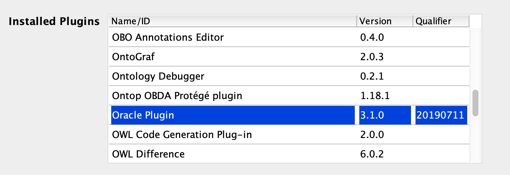
\includegraphics[width=0.7\linewidth]{imagenes/apendices/Imagen1}
	\caption{Comprobación del Plugin Oracle Database instalado}
	\label{fig:imagen1-comprobar}
\end{figure}

\begin{figure}[H]
	\centering
	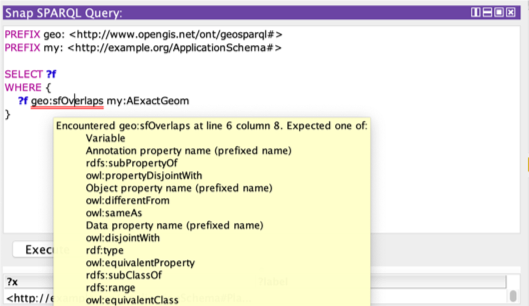
\includegraphics[width=0.8\linewidth]{imagenes/apendices/Imagen2}
	\caption{Error de GeoSPARQL en Protegé}
	\label{fig:imagen2-error}
\end{figure}

Por otro lado, para asegurarme de que la consulta de GeoSPARQL en Protegé que estaba realizando era correcta he cogido un ejemplo proporcionado por el organismo de estándares OGC (\url{https://www.opengeospatial.org/standards/geosparql}) y al probarlo en otra herramienta he verificado que funcionaba. Pero al no conseguir éxito en Protegé, he buscado otros softwares que me permitieran hacer uso de GeoSPARQL.

\begin{figure}[H]
	\centering
	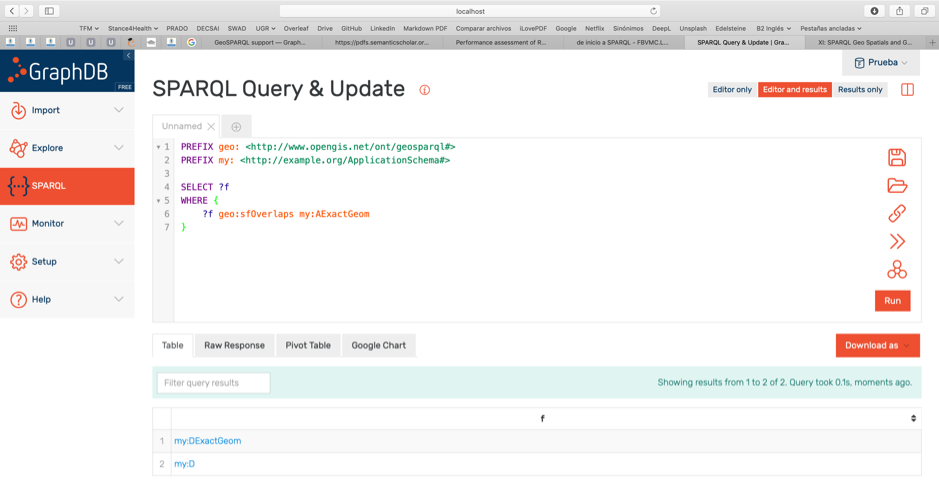
\includegraphics[width=1\linewidth]{imagenes/apendices/Imagen3}
	\caption{Comprobación del funcionamiento de GeoSPARQL en GraphDB}
	\label{fig:imagen3-funciona}
\end{figure}


He estado buscando en Internet qué herramientas son aconsejables para hacer uso de GeoSPARQL, y he encontrado que la más se repetía era \textbf{GraphDB} (\url{https://www.ontotext.com/products/graphdb/#Try-GraphDB}) y además, es una de las que aconseja la página de Wikipedia (\url{https://en.wikipedia.org/wiki/OGC_GeoSPARQL}). Por eso mismo me he descargado la versión gratuita del programa y me lo he instalado (se necesita tener Java instalado con una determinada versión y requisitos especiales), al instalarse se abre en un servidor, por lo que todo se maneja desde el navegador y he probado el ejemplo (\url{http://graphdb.ontotext.com/documentation/standard/geosparql-support.html#plugin-control-predicates}) y con GRAPHDB sí que ha funcionado (figura \ref{fig:imagen3-funciona}). En el \texttt{Apéndice C: Instalación de GraphDB} es posible ver la instalación de este software.\\


%Sin embargo, para hacer uso de GeoSPARQL todos hacen uso de ficheros “.rdf” y no de ficheros “.owl”, no sé si eso tiene algo que ver o si dificulta, el único problema que yo crearía la ontología con Protegé, pero no me deja sacar la salida para RDF, sino es para OWL. De todas maneras el contenido del fichero para obtener esa salida anterior es (geosparql-example.rdf). Qué según veo mete los datos distintos a como los estaba metiendo yo, ya que tendría que sacar las coordenadas de los polígonos, puntos y líneas para meterlos dentro.

No obstante, durante la búsqueda de alternativas a Protegé para GeoSPARQL he encontrados otras herramientas, pero debido a su dificultad he terminado por escoger la que acaba de exponer.

